\documentclass[../main.tex]{subfiles}

\begin{document}
\section{Preliminaries}\label{sec:preliminaries}
In this section we will review some basic concepts of linear algebra and vector calculus that will be used throughout the document.
\subsection{Properties of cross and dot products}
\begin{proposition}
  \label{prop:triplecross}
  Let $\vf{u}, \vf{v}, \vf{w}\in\RR^3$. Then:
  \begin{align}
    (\vf{u}\times\vf{v})\times\vf{w} & =(\vf{u}\cdot\vf{w})\vf{v}-(\vf{v}\cdot\vf{w})\vf{u} \\
    \vf{u}\times(\vf{v}\times\vf{w}) & =(\vf{u}\cdot\vf{w})\vf{v}-(\vf{u}\cdot\vf{v})\vf{w}
  \end{align}
\end{proposition}
\begin{proof}
  Let $\vf{u}=(u_1,u_2,u_3)$, $\vf{v}=(v_1,v_2,v_3)$, and $\vf{w}=(w_1,w_2,w_3)$. Then:
  \begin{align*}
    {((\vf{u}\times\vf{v})\times\vf{w})}_1 & =(u_3v_1-u_1v_3)w_3-(u_1v_2-u_2v_1)w_2                     \\
                                           & =(u_2w_2+u_3w_3)v_1-(v_2w_2+v_3w_3)u_1                     \\
                                           & =(u_1w_1+u_2w_2+u_3w_3)v_1-(v_1w_1+v_2w_2+v_3w_3)u_1       \\
                                           & ={((\vf{u}\cdot\vf{w})\vf{v}-(\vf{v}\cdot\vf{w})\vf{u})}_1
  \end{align*}
  The other components are treated similarly. The second equality follows in a similar way.
\end{proof}
\begin{proposition}
  Let $\vf{u}, \vf{v}, \vf{w}\in\RR^3$. Then:
  \begin{enumerate}
    \item $(\vf{u}\times\vf{v})\cdot\vf{w}=(\vf{u}\cdot\vf{w})\vf{v}\cdot\vf{w}-(\vf{v}\cdot\vf{w})\vf{u}\cdot\vf{w}$
  \end{enumerate}
\end{proposition}
\subsection{Conics in a nutshell}
\begin{definition}
  A conic is the curve obtained as the intersection of a plane with the surface of a double cone (a cone with two \emph{nappes}).
\end{definition}
In \cref{fig:conics}, we show the 3 types of conics: the ellipse, the parabola, and the hyperbola, which differ on their eccentricity, as we will see later. Note that the circle is a special case of the ellipse.
\begin{figure}[htbp]
  \centering
  \begin{minipage}[t]{0.45\textwidth}
    \centering
    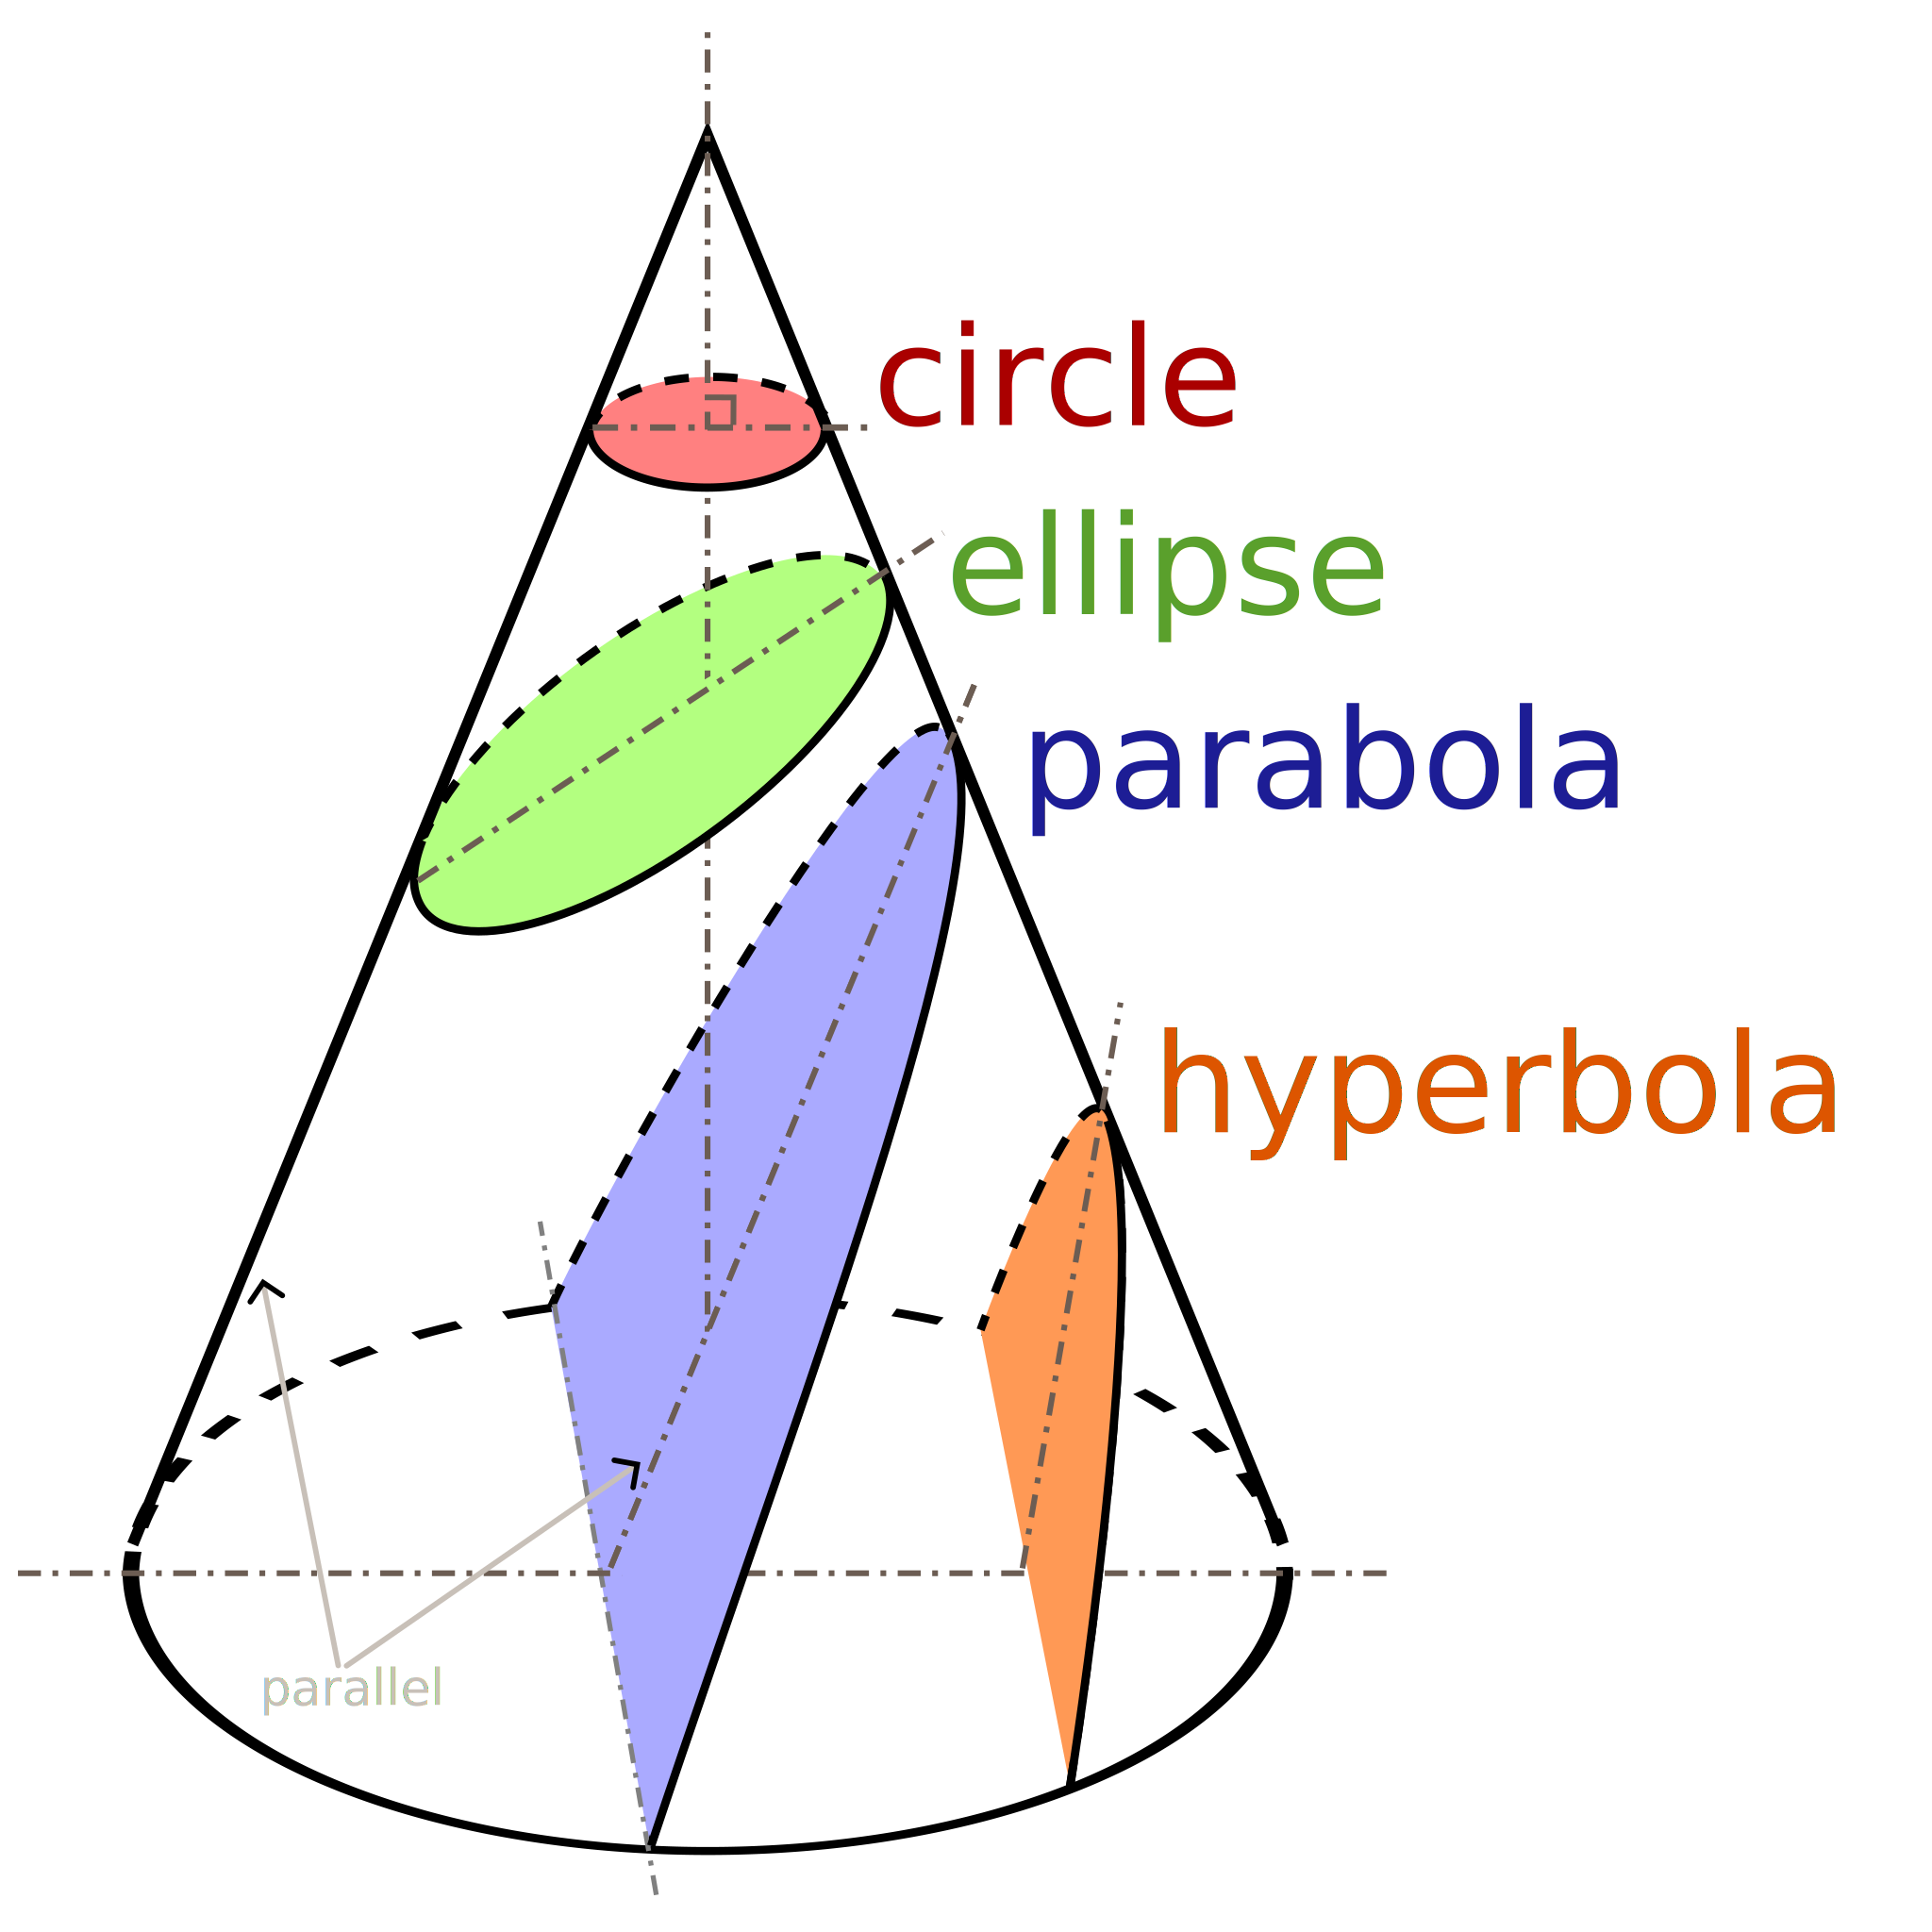
\includegraphics[width=\textwidth]{Images/Conic_Sections.pdf}
    \caption{The black boundaries of the colored regions are conic sections. The other half of the hyperbola, which is not shown, is the other nappe of the double cone.}
    \label{fig:conics}
  \end{minipage}
  \hfill
  \begin{minipage}[t]{0.45\textwidth}
    \centering
    \includegraphics[width=\textwidth]{Images/conics.pdf}
    \caption{Reference frame centered at the focus of the conic and whose axes are such that the $y$-axis is parallel to the directrix and the $x$-axis is perpendicular to the directrix. The directions of the axes are chosen arbitrarily, subject to the constraint that a positive basis is chosen.}
    \label{fig:conics_cartesian}
  \end{minipage}
\end{figure}
\begin{definition}
  The \emph{locus} is a set of points that satisfy a given condition.
\end{definition}
The following proposition gives a characterization of the conics.
\begin{proposition}
  A conic is the locus of all points $P$ such that the distance from $P$ to a fixed point $F$ is a multiple of the distance from $P$ to a fixed line $D$. Mathematically, this is expressed as:
  \begin{equation}\label{eq:conic_pre}
    d(P,F)=e d(P,D)
  \end{equation}
  where $d$ is the Euclidean distance. The point $F$ is called the \emph{focus}; the line $D$, \emph{directrix}, and the constant of proportionality $e$, \emph{eccentricity}.
\end{proposition}
Note that using the polar coordinates $(r,\nu)$ as in \cref{fig:conics_cartesian}, we can rewrite \cref{eq:conic_pre} as:
\begin{equation}\label{eq:conic}
  r=e(\ell - r\cos\nu)\implies r= \frac{e\ell}{1+e\cos\nu}=:\frac{p}{1+e\cos\nu}
\end{equation}
where we have defined $p:=e\ell$.
\begin{definition}
  Le $C$ be a conic and $e$ be its eccentricity. We say that $C$ is
  \begin{itemize}
    \item an \emph{ellipse} if $0\leq e<1$,
    \item a \emph{parabola} if $e=1$, and
    \item a \emph{hyperbola} if $e>1$.
  \end{itemize}
  If $e=0$, the conic is a \emph{circle}.
\end{definition}
\subsection{Spherical harmonics}
\subsubsection{Legendre polynomials, regularity and orthonormality}
\begin{definition}
  \textcolor{red}{Consider the following second-order differential equation:
    \begin{equation}
      y''+p_1(x)y'+p_0(x)y=0
    \end{equation}
    We say that $a$ is an \emph{ordinary point} if $p_1$ and $p_2$ are analytic at $x=a$. We say that $a$ is a \emph{regular singular point} if $p_1$ has a pole up to order 1 at $a$ and $p_0$ has a pole of order up to 2 at $a$. Otherwise we say that $a$ is a \emph{irregular singular point}.}
\end{definition}
\begin{definition}
  Consider the following second-order differential equation called \emph{Legendre differential equation}:
  \begin{equation}
    (1-x^2)y''-2xy'+\lambda y=0
  \end{equation}
  for $n\in\NN\cup\{0\}$. This equation can be written as:
  \begin{equation}\label{eq:legendre_diff_eq}
    {((1-x^2)y')}'+\lambda  y=0
  \end{equation}
\end{definition}
If seek for analytic solutions of this equation using the power series method, i.e. looking for solutions of the form $y(x)=\sum_{j=0}^{\infty}a_jx^j$ one can check that we obtain this recursion:
\begin{equation}\label{eq:legendre_recursion}
  a_{j+2}=\frac{j(j+1)-\lambda}{(j+1)(j+2)}a_j\quad j=0,1,2,\ldots
\end{equation}
From here we can obtain two independent solutions by setting the initial conditions $a_0$ and $a_1$ of the iteration. For example, setting $a_1=0$ we obtain a series that has only even powers of $x$. On the other hand, setting $a_0=0$ we obtain a series that has only odd powers of $x$. These two series converge on the interval $(-1,1)$ by the ratio test (by looking at \cref{eq:legendre_recursion}) and can be expressed compactly as \cite{florida:legendre}:
\begin{equation}\label{eq:legendre_series}
  y_\mathrm{e}(x)=a_0\sum_{j=0}^{\infty}\left[\prod_{k=0}^{j-1}(2k(2k+1)-\lambda)\right]\frac{x^{2j+1}}{(2j)!}\qquad y_\mathrm{o}(x)=a_1\sum_{j=0}^{\infty}\left[\prod_{k=1}^j(2k(2k+1)-\lambda)\right]\frac{x^{2j+1}}{(2j+1)!}
\end{equation}
However either for all $\lambda\in\RR$ either one of these series diverge at $x=\pm 1$, as it behaves as the harmonic series in a neighbourhood of $\pm 1$. We are interested, though, in the solutions that remain bounded on the whole interval $[-1,1]$. Looking at the expressions of \cref{eq:legendre_series} one can check that the only possibility to make the series converge on $[-1,1]$ is when $\lambda =n(n+1)$, $n\in\NN\cup\{0\}$. In this case, either one of the series is in fact a polynomial. In both cases it reduces to a polynomial of degree $n$. For each $n\in\NN\cup\{0\}$ if we choose $a_0$ or $a_1$ be such that the polynomial evaluates to 1 at $x=1$, these polynomials are called \emph{Legendre polynomials} and they are denoted by $P_n(x)$. The other (divergent) series is usually denoted in the literature by $Q_n(x)$ (check \cite{mathematical_methods}). And so the general solution of \cref{eq:legendre_diff_eq} for $\lambda=n(n+1)$ can be expressed as a linear combination of $P_n$ and $Q_n$.

\begin{figure}[htbp]
  \centering
  \begin{minipage}[ht]{0.45\textwidth}
    \centering
    \includegraphics[width=\textwidth]{Images/legendre.pdf}
    \caption{Graphic representation of the first eight Legendre polynomials.}
  \end{minipage}
  \hfill
  \begin{minipage}[ht]{0.45\textwidth}
    \centering
    \captionsetup{type=table} %% tell latex to change to table
    \begin{tabular}{c|c}
      $n$ & $P_n(x)$                                 \\
      \hline\hline
      $0$ & $1$                                      \\
      $1$ & $x$                                      \\
      $2$ & $\frac{1}{2}(3x^2-1)$                    \\
      $3$ & $\frac{1}{2}(5x^3-3x)$                   \\
      $4$ & $\frac{1}{8}(35x^4-30x^2+3)$             \\
      $5$ & $\frac{1}{8}(63x^5-70x^3+15x)$           \\
      $6$ & $\frac{1}{16}(231x^6-315x^4+105x^2-5)$   \\
      $7$ & $\frac{1}{16}(429x^7-693x^5+315x^3-35x)$ \\
    \end{tabular}
    \caption{First eight Legendre polynomials}
    \label{tab:legendre_polys}
  \end{minipage}
\end{figure}
\textcolor{red}{\begin{proposition}
    Consider the function $g_x(t)=\frac{1}{\sqrt{1-2xt+t^2}}$ with $\abs{x}\leq 1$. Then, the generating function of $g$ is:
    \begin{equation}
      \frac{1}{\sqrt{1-2xt+t^2}}=\sum_{n=0}^{\infty}P_n(x)t^n
    \end{equation}
  \end{proposition}
  \begin{proof}
    Assume that formally $\frac{1}{\sqrt{1-2xt+t^2}}=\sum_{n=0}^{\infty}Q_n(x)t^n$. We want to check that $Q_n(x)=P_n(x)$ for all $n\in\NN\cup\{0\}$. Differentiating the equation with respect to $x$ and with respect to $t$ we obtain:
    \begin{equation}\label{eq:rec_legendre_proof}
      \frac{x-t}{{(1-2xt+t^2)}^{3/2}}=\sum_{n=0}^{\infty}nQ_n(x)t^{n-1}\qquad\frac{t}{{(1-2xt+t^2)}^{3/2}}=\sum_{n=0}^{\infty}{Q_n}'t^n
    \end{equation}
    The second equation can be rewritten as:
    \begin{equation}
      t\sum_{n=0}^{\infty}Q_n t^n=(1-2xt+t^2)\sum_{n=0}^{\infty}{Q_n}'(x)t^{n-1}
    \end{equation}
    So equating the coefficients of $t^n$ we get:
    \begin{equation}
      Q_{n}={Q_{n+1}}'-2x{Q_n}'+{Q_{n-1}}'
    \end{equation}
    Moreover, from \cref{eq:rec_legendre_proof} we have that:
    \begin{equation}
      t\sum_{n=0}^{\infty}nQ_n(x)t^{n-1}=(x-t)\sum_{n=0}^{\infty}{Q_n}'(x)t^{n}
    \end{equation}
    Again equating the coefficients of $t^n$ we get:
    \begin{equation}
      nQ_n=x{Q_n}'-{Q_{n-1}}'
    \end{equation}
    Hence differentiating $(1-x^2){P_n}'$ we have:
    \begin{equation}
      {((1-x^2){P_n}')}'=-2x{P_n}'+(1-x^2)P
    \end{equation}
    \textcolor{red}{NOT FINISHED!!!!!!!!!!}
  \end{proof}}
\begin{proposition}\label{prop:associate_legendre}
  Let $y(x)$ be a solution to the Legendre differential equation. Then, $\forall m\in\ZZ$ the function
  \begin{equation}
    w_m(x)={(1-x^2)}^{m/2} \dv[m]{y(x)}{x}
  \end{equation}
  solves the \emph{general Legendre differential equation}:
  \begin{equation}
    (1-x^2)y''-2xy'+\left(\lambda - \frac{m^2}{1-x^2}\right) y=0
  \end{equation}
  In particular if $\lambda=n(n+1)$ for $n\in\NN\cup\{0\}$, then $w_m(x)$ is denoted as
  \begin{equation}
    P_n^m(x):={(1-x^2)}^{m/2} \dv[m]{P_n}{x}
  \end{equation}
  and it is called the \emph{associated Legendre polynomial} of degree $n$ and order $m$.
\end{proposition}
Note that although these functions $P_n^m$ are referred to \emph{polynomials}, they are only \emph{real} polynomials if $m$ is even. But we have opt to call them as it is the common practice in the literature (see \cite{wolfram_associated_legendre_polynomials}).

Moreover, from the definition of $P_n^m$, we can see $P_n^0=P_n$ and that $P_n^m=0$ if $m>n$. So we can restrict the domain of $m$ to the set $\{0,1,\dots,n-1,n\}$.

\begin{definition}
  Let $n\in\NN\cup\{0\}$ and $m\in\{0,1,\dots,n-1,n\}$. We define the \emph{spherical harmonic} $Y_n^m$ as:
  \begin{equation}
    Y_n^m(\theta,\phi)=P_n^{\abs{m}}(\cos\phi) \exp{\ii m\theta}
  \end{equation}
\end{definition}
\subsubsection{Laplace equation in spherical coordinates}\label{sec:laplace_spherical}
\begin{definition}
  Let $f:\RR^3\rightarrow\RR$ be a twice-differentiable function. The \emph{Laplace equation} is the equation
  \begin{equation}
    \laplacian f=\pdv[2]{f}{x}+\pdv[2]{f}{y}+\pdv[2]{f}{z}=0
  \end{equation}
  where $\Delta$ is the Laplace operator.
\end{definition}
The next proposition gives the Laplace equation in spherical coordinates.
\begin{proposition}
  Let $f:\RR^3\rightarrow\RR$ be a twice-differentiable function. Then:
  \begin{equation}\label{eq:laplace}
    \frac{1}{r^2}\pdv{}{r}\left(r^2\pdv{f}{r}\right)+\frac{1}{r^2\sin\phi}\pdv{}{\phi}\left(\sin\phi\pdv{f}{\phi}\right)+\frac{1}{r^2{(\sin\phi)}^2}\pdv[2]{f}{\theta}=0
  \end{equation}
  where $r$ denotes the radial distance, $\theta$ denotes the azimuthal angle, and $\phi$, the polar angle.
\end{proposition}
Recall that a solutions to the \emph{Dirichlet problem} on a bounded domain $\Omega\subset\RR^3$
\begin{equation}
  \begin{cases}
    \laplacian u=0 & \text{in } \Omega         \\
    u=g            & \text{on } \partial\Omega
  \end{cases}
\end{equation}
exists and is unique if $g$ is sufficiently smooth. \cref{thm:laplace_spherical} gives them as a function of the so-called
\begin{theorem}\label{thm:laplace_spherical}
  The regular solutions in a bounded region $\Omega\subseteq \RR^3$ such that $0\notin\overline{\Omega}$ to the Laplace equation in spherical coordinates are of the form
  \begin{equation}\label{eq:sol_laplace}
    f(r,\theta,\phi) = \sum_{n=0}^\infty \sum_{m=-n}^n (c_{n}^m r^{n} +d_n^mr^{-n-1})P_n^\abs{m}(\cos\phi) \exp{\ii m\theta}= \sum_{n=0}^\infty \sum_{m=-n}^n (c_{n}^m r^{n} +d_n^mr^{-n-1})Y_n^m(\theta,\phi)
  \end{equation}
  where $c_{n}^m,d_n^m\in\CC$.
\end{theorem}
\begin{proof}
  Let $f(r,\theta,\phi)$ be a solution of \cref{eq:laplace} Using separation variables $f(r,\theta,\phi)=R(r)\Theta(\theta)\Phi(\phi)$ one can write:
  \begin{equation}
    \frac{\Theta\Phi}{r^2}{(r^2R')}'+\frac{R\Theta}{r^2\sin\phi}{(\sin\phi\Phi')}'+\frac{R\Phi}{r^2{(\sin\phi)}^2}\Theta''=0
  \end{equation}
  Isolating $R$ from $\Theta$ and $\Phi$ yields:
  \begin{equation}
    \frac{{(r^2R')}'}{R}=-\frac{1}{\sin\phi\Phi}{(\sin\phi\Phi')}'-\frac{1}{{(\sin\phi)}^2\Theta}\Theta''
  \end{equation}
  Since the left-hand side depends entirely on $r$ and the right-hand side does not, we must need that both sides are constant. Hence:
  \begin{align}
    \label{eq:laplaceR}        & \frac{{(r^2R')}'}{R}=\lambda                                                               \\
    \label{eq:laplaceThetaPhi} & \frac{1}{\sin\phi\Phi}{(\sin\phi\Phi')}'+\frac{1}{{(\sin\phi)}^2\Theta}\Theta''  =-\lambda
  \end{align}
  with $\lambda\in\RR$. Similarly from \cref{eq:laplaceThetaPhi} we obtain that the equations
  \begin{align}
    \label{eq:laplaceTheta} & \frac{1}{\Theta}\Theta''  =-m^2                                     \\
    \label{eq:laplacePhi}   & \frac{\sin\phi}{\Phi}{(\sin\phi\Phi')}'+\lambda{(\sin\phi)}^2  =m^2
  \end{align}
  must be constant with $m\in\CC$ (a priori). The solution to \cref{eq:laplaceTheta} is a linear combination of the exponentials $\exp{\ii m\theta}$, $\exp{-\ii m\theta}$. Note, though, that since $\Theta$ must be a $2\pi$-periodic function, that is satisfying $\Theta(\theta+2\pi)=\Theta(\theta)$ $\forall\theta\in\RR$, $m$ must be an integer. On the other hand making the change of variables $x=\cos \phi$ and $y=\Phi(\phi)$ in \cref{eq:laplacePhi}, that equation becomes:
  \begin{equation}
    (1-x^2)\dv[2]{y}{x}-2x\dv[2]{y}{x}+\left(\lambda-\frac{m^2}{1-x^2}\right)y=0
  \end{equation}
  which is the associate Legendre equation. We have argued in \cref{prop:associate_legendre} that we need $\lambda=n(n+1)$ and $m\leq n$ in order to get regular solutions at $x=\cos\phi=\pm 1$. Moreover these solutions are $P_n^m(\cos\phi)$.

  Finally note that equation \cref{eq:laplaceR} is a Cauchy-Euler equation (check \cite{wiki:cauchy-euler}) and so it general solution is given by
  \begin{equation}
    R(r) = c_1 r^{n} + c_2 r^{-n-1}
  \end{equation}
  because $\lambda = n(n+1)$. So the general solution becomes a linear combination of the each solution founded varying $n\in\NN\cup\{0\}$ and $m\in\{0,1,\dots,n-1,n\}$:
  \begin{equation}
    f(r,\theta,\phi) = \sum_{n=0}^\infty \sum_{m=-n}^n (c_{n}^m r^{n} +d_n^mr^{-n-1})P_n^\abs{m}(\cos\phi) \exp{\ii m\theta}
  \end{equation}
\end{proof}
From now we are not concerning of the singularity at $r=0$ of \cref{eq:sol_laplace} (see SECTION-POTENTIAL for more details).

With a bit of patience one can prove that $\forall n_1,n_2\in\NN\cup\{0\}$ and all $0\leq m\leq\min\{n_1,n_2\}$:
\begin{equation}
  \int_0^1 P_{n_1}^{m}(x) P_{n_2}^{m}(x) \dd{x}=\frac{2}{2n+1}\frac{(n+m)!}{(n-m)!} \delta_{n_1,n_2}
\end{equation}
where $\delta_{n_1,n_2}$ denotes the Kronecker delta.
From here it's not hard to prove that the spherical harmonics behave in a similar way:
\begin{equation}
  \int_0^{2\pi}\int_0^\pi Y_{n_1}^{m_1}(\theta,\phi) \overline{Y_{n_2}^{m_2}(\theta,\phi)} \dd{\phi}\dd{\theta}=\frac{2}{2n+1}\frac{(n+m)!}{(n-m)!} \delta_{n_1,n_2}\delta_{m_1,m_2}
\end{equation}

Moreover, an important result in the Sturm-Liouville Theory of second order differential equations (\cite{wiki:sturm-liouville,completeness_SL}) says that the family of spherical harmonics $\{Y_n^m(\theta,\phi):n\in\NN\cup\{0\},\abs{m}\leq n\}$ form a complete set in the sense that any smooth function defined on the sphere $f:S^2\rightarrow\RR$ can be expanded in a series of spherical harmonics:
\begin{equation}
  f(\theta,\phi)=\sum_{n=0}^\infty\sum_{m=-n}^n c_{n}^m Y_n^m(\theta,\phi)
\end{equation}
\end{document}